\documentclass[10pt,twocolumn,letterpaper]{article}

\usepackage[hangul]{kotex}
\usepackage{times}
\usepackage{epsfig}
\usepackage{graphicx}
\usepackage{amsmath}
\usepackage{amssymb}
\usepackage{url}
\usepackage{algorithm}% http://ctan.org/pkg/algorithms
\usepackage[noend]{algpseudocode}% http://ctan.org/pkg/algorithmicx
\usepackage{subcaption}

\usepackage[breaklinks=true,bookmarks=false]{hyperref}

\begin{document}

\title{Maximum flow와 관련 내용들}
\author{김찬민}

\maketitle

경기 프로그래밍 분야에서 잘 알려진 내용들 수집하고 정리한 것이다.

\section{Notations}

$G=(V,E)$는 그래프 또는 네트워크를 의미한다. $V$와 $E$는 각각 정점과 간선이다.

$u$, $v$, $w$는 보통 정점(vertex)을 나타낸다.
$s$는 시작 정점(source), $t$는 도착 정점(sink)을 나타낸다.

$u \rightarrow v$는 $u$에서 $v$로 가는 방향의 간선(edge)를 의미한다.

$c_{u \rightarrow v}$는 $u$에서 $v$로 가는 간선의 capacity를 나타낸다.
$f_{u \rightarrow v}$는 $u$에서 $v$로 가는 간선에 흐르는 flow를 나타낸다.
$r_{u \rightarrow v}$는 $u$에서 $v$로 가는 간선의 residual capacity를 나타낸다.

\section{Maximum Flow}

\subsection{Vertex Capacity}

vertex capacity는 vertex마다 허용되는 유량의 최대치가 있는 경우이다.  vertex $v$의 capacity를 $v_c$라 하자.

vertex $v$를 제거하고, $v_{in}$과 $v_{out}$을 추가한다.
$c_{u \rightarrow v}$마다 $c_{u \rightarrow v_{in}}$인 간선을 추가한다.
$c_{v \rightarrow w}$마다 $c_{v_{out} \rightarrow w}$인 간선을 추가한다.
$c_{v_{in} \rightarrow v_{out}}$ = $c_{v}$로 하여 간선을 추가한다.

직관적으로는 vertex를 두 개로 쪼개고, 사이에 edge를 추가하여 그 edge가 vertex capacity를 담당하도록 한 것이다.

\begin{figure}
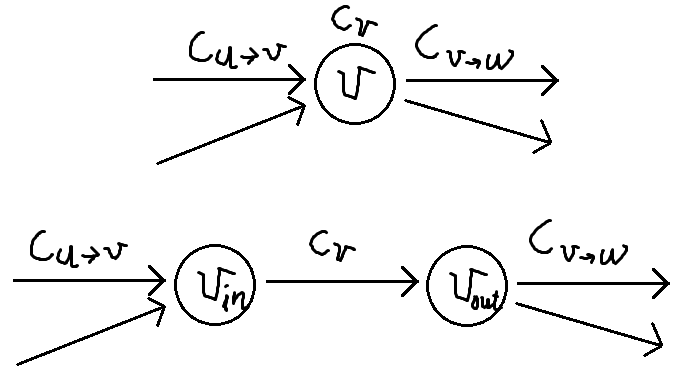
\includegraphics[width=0.9\linewidth]{vertex_doubling.png}
\caption{vertex capacity 적용 그림}
\end{figure}


\subsection{Dilworth's Theorem}

\subsection{Kőnig's Theorem}

이분 그래프(bipartite graph)에서, maximum matching과 minimum vertex cover는 같다.

$L$과 $R$의 두 정점 집합이 있다고 하자. unmatched 간선은 $L \rightarrow R$로 가도록 방향을 잡는다. matched 간선은 $R \rightarrow L$로 가도록 방향을 잡는다.
여기서 $L$의 원소들 중, match되지 않은 정점들로부터 출발해서 도달 가능한 모든 정점을 체크한다.
$L$에서 체크되지 않은 정점들(nocheck)과 $R$에서 체크된 정점들(check)이 vertex cover이다.

우선 매칭된 간선이 잇는 $L$과 $R$의 정점은 둘 다 check거나, 둘 다 nocheck거나 두가지 중 하나이다.
나머지 간선이 check $\rightarrow$ nocheck로  가는 것은 불가능하다.
check에서 출발하는 경우, check에 도달하므로 $R$의 check가 cover한다.
nocheck에서 출발하는 경우, $L$의 nocheck가 cover한다.
따라서 이 방법으로 구한 것은 vertex cover이다.

이제 minimum인 이유이다. matching된 간선들만 놓았을 때, 겹치는 vertex가 없으므로, 적어도 matching된 간선의 개수만큼은 있어야 cover가 가능하다.

\subsection{Maximum Flows with Edge Demands}

최소 유량 조건이 붙어있는 확장이다. 주어진 demand $d$와 capacity $c$에 대해, flow $f$는 $d_i \le f_i \le c_i$를 만족해야 한다.

가짜 vertex $s'$과 $t'$을 만든다.

\section{Minimum Cut}

\subsection{Project Selection}

\subsection{cut의 weight가 여러가지 있는 경우}

capacity가 tuple이 된다.
예를 들어, 최소 가중치 컷 중에서도, 최소 개수의 간선 컷을 찾고 싶다면 가중치 $w$가 $(w, 1)$이 된다.
이 때 비교 연산은 lexicographical order로 하고, $0$은 $(0, 0)$이 된다. 덧셈과 뺄셈 연산은 벡터 연산처럼 각 차원마다 적용한다.

\subsection{Maximum Closure Problem}

\section{Minimum Cost Flow}


\section{Marriage Problem}

\section{Birkhoff–von Neumann Theorem}

간단히 얘기해서, 임의의 행/열 합이 같은 매트릭스는 항상 permutation matrix(perfect matching)으로 분리해낼 수 있다는 정리이다.
실제로 답을 구하려면 zero/nonzero 구분한 이진매트릭스에서 계속 perfect matching 아무거나 찾아주면 된다.
정수 행렬일 때는 정수 계수 permutation matrix 분해가 가능하다.

https://math.stackexchange.com/a/583999
mentioning Hall's condition


\end{document}
